\documentclass[reprint, aps, pra, twocolumn, superscriptaddress, floatfix]{revtex4-2}

\usepackage[utf8]{inputenc}
\usepackage{amsmath}
\usepackage{amssymb}
\usepackage{graphicx}
\usepackage{xcolor}
\usepackage{braket}
\usepackage{microtype}
\usepackage{bm}
\usepackage{pgfplots}
\pgfplotsset{compat=1.18}

\usepackage{orcidlink}
\usepackage{hyperref}


% Define the sign operator
\DeclareMathOperator{\sign}{sign}

\hypersetup{
    colorlinks=true,
    linkcolor=blue,
    citecolor=blue,
    urlcolor=blue,
    pdftitle={Quantum Clocks Tick Faster},
    pdfauthor={Karl Svozil}
}

\begin{document}

\title{Quantum Clocks Tick Faster: Entanglement, Contextuality, and the Flow of Time}

\author{Karl Svozil\,\orcidlink{0000-0001-6554-2802}}
\email{karl.svozil@tuwien.ac.at}
\homepage{http://tph.tuwien.ac.at/~svozil}

\affiliation{Institute for Theoretical Physics,
TU Wien,
Wiedner Hauptstrasse 8-10/136,
1040 Vienna,  Austria}

\date{\today}

\begin{abstract}
Building on the recent proposal that a single ``bona fide'' clock suffices to define spacetime's metric, we introduce an \emph{Entangled Clock} protocol based on singlet-state correlations. Invoking Zeilinger's Foundational Principle, we argue that while the local flow of time, operationally defined as a sequence of detector ``ticks,'' is irreducibly random (one bit per elementary system), the synchronized flow between spatially separated observers depends on their measurement geometry. Comparing the quantum prediction for the coincidence rate with Peres' classical ``bomb fragment'' model, we find that at obtuse relative angles ($\theta \approx 140^\circ$) the entangled clock exhibits a ${\sim}13\%$ higher synchronized tick rate than this linear classical benchmark. This ``temporal acceleration'' is linked to contextuality: following Peres, ``unperformed experiments have no results,'' and quantum systems are not constrained to maintain consistency with all counterfactual measurement settings. We stress, however, that for any \emph{single} measurement angle a suitably tailored classical model can reproduce the quantum rate. The genuinely nonclassical character of the entangled clock emerges only when correlations at several angles are considered simultaneously and are shown to violate Bell-type inequalities. In this sense, the violation of Bell-type bounds serves as a certification that the shared time standard is genuinely quantum.
\end{abstract}

\maketitle

\section{Introduction}

The question of the fundamental nature of time and its measurement has recently been revisited through two distinct but complementary lenses: operational metrology in relativity and information-theoretic constraints in quantum foundations.

On the metrological side, the ``trialogue'' regarding the number of fundamental constants~\cite{DuffOkunVeneziano} established a consensus that dimensionless quantities are the ultimate observables. More recently, Matsas, Pleitez, Saa, and Vanzella~\cite{matsas-2024} argued that a relativistic spacetime requires only a single fundamental dimensional constant. By employing ``bona fide clocks,'' one can define the spacetime metric entirely through proper time measurements, rendering spatial rulers redundant.
This ``single-unit universe''---a cosmos whose metric geometry is fixed by
a single dimensional constant, namely proper time---relies on the mathematical rigidity of the Alexandrov-Zeeman theorems~\cite{alex3,zeeman}. These theorems state that the causal structure (light cones) determines the geometry of Minkowski spacetime up to a global conformal factor. The physical clock breaks this dilation symmetry, fixing the scale of the universe~\cite{svozil-2025-lt}.

If a single clock fixes the scale of the universe, a natural question arises: how do two such clocks, spatially separated but sharing a quantum history, measure the flow of time relative to one another? In classical relativity, synchronization is a matter of signaling and convention (Einstein synchronization~\cite{ein-05}). In quantum mechanics, by contrast, synchronization can be mediated by entanglement, which introduces nonclassical correlations between distant systems. These correlations are constrained by no-go theorems such as Bell's, and thus cannot in general be accounted for by local realistic statistics.

This brings us to the second lens: the study of quantum correlations. Zeilinger~\cite{zeil-99} proposed a foundational principle: that the irreducible randomness of quantum events arises because an elementary system carries only one bit of information. In an entangled state, this information is exhausted by the joint properties, leaving the individual constituents completely undefined. Simultaneously, Peres~\cite{peres222} demonstrated that classical correlations are strictly bounded because one can validly imagine the results of ``unperformed experiments.'' In contrast, quantum correlations defy these bounds precisely because such counterfactuals are illegitimate.

In this paper, we unify these perspectives to propose the concept of an \emph{Entangled Clock}. We define the ``tick'' of a clock operationally as the registration of a measurement outcome. We show that the synchronization rate of two such clocks is not merely a function of relativistic geometry, but of the information-theoretic constraints on the system. By comparing the quantum prediction against Peres' classical linear model, we identify a regime where the quantum clock ``ticks faster'' (shows higher coincidence rates) than this natural classical benchmark and, when correlations at several angles are taken into account, faster than any local realistic model allows.

\section{The Entangled Clock Protocol}

We construct a distributed time standard using a sequence of bipartite quantum systems. Let a source emit pairs of spin-1/2 particles (or polarization-entangled photons) in the singlet Bell state $\ket{\psi^-}$:
\begin{equation}
\ket{\psi^-} = \frac{1}{\sqrt{2}} \left( \ket{+}_A \ket{-}_B - \ket{-}_A \ket{+}_B \right),
\end{equation}
where $A$ and $B$ denote two spatially separated observers (Alice and Bob). Each observer possesses a measurement apparatus oriented along directions defined by unit vectors $\vec{a}$ and $\vec{b}$, respectively.

\subsection{Operational Time and Zeilinger's Principle}

We define operational time $T$ on each side not as a continuous background parameter, but as the accumulation of discrete events. Specifically, whenever a detector records a specific outcome (say, ``up'' or $+1$), the local clock increments by one unit:
\begin{equation}
T_i \to T_i + 1 \quad \text{if } \sigma_i = +1, \quad i \in \{A, B\}.
\end{equation}
If the outcome is ``down'' ($-1$), the clock implies a ``pause'' or a non-tick for that interval.

According to Zeilinger's Foundational Principle~\cite{zeil-99}, an elementary system represents the truth value of a single proposition (1 bit). For a composite system of two spin-1/2 particles, the total information capacity is 2 bits. In the singlet state $\ket{\psi^-}$, these 2 bits are entirely exhausted by the joint propositions (e.g., ``spins are opposite along $z$'' and ``spins are opposite along $x$''). Consequently, the system contains \emph{zero} information about individual properties along any specific direction $\vec{n}$.
\begin{equation}
P(+)_{\vec{n}} = P(-)_{\vec{n}} = \frac{1}{2}.
\end{equation}
Thus, the \emph{local} proper time measured by Alice or Bob flows stochastically. Over a large ensemble of $N$ pairs, the local clock will record approximately $N/2$ ticks. This randomness is not merely epistemic; it is ontologically necessary because the individual particle carries no answer to the question ``are you up or down?'' until the measurement is performed.

\subsection{Synchronized Time}

While local time is random, the relative time evolution between Alice and Bob is structured by entanglement. We define the \emph{synchronized time rate} $R(\theta)$ as the probability that both clocks tick simultaneously in a given run (a coincidence count).
\begin{equation}
R(\theta) = P_{++}(\vec{a}, \vec{b}),
\end{equation}
where $\theta$ is the angle between the measurement vectors $\vec{a}$ and $\vec{b}$.

For the singlet state, quantum mechanics predicts the joint expectation value $E_{QM}(\theta) = \braket{\sigma_{\vec{a}} \otimes \sigma_{\vec{b}}} = -\vec{a}\cdot\vec{b} = -\cos\theta$. The probability of a coincident tick ($+1, +1$) is derived as follows:
\begin{align}
R_{QM}(\theta) &= \frac{1}{4} \left( 1 + \braket{\sigma_A} + \braket{\sigma_B} + \braket{\sigma_A \sigma_B} \right) \nonumber \\
&= \frac{1}{4} \left( 1 + 0 + 0 - \cos\theta \right) \nonumber \\
&= \frac{1}{2}\sin^2\frac{\theta}{2}.
\label{eq:qm_rate}
\end{align}

\textit{Implementation Note:} While we describe the protocol using spin-1/2 particles, an equivalent implementation uses polarization-entangled photon pairs. In that case, $\ket{+}/\ket{-}$ correspond to horizontal/vertical polarizations, and the detectors are linear polarizers. A ``tick'' corresponds to a photon passing through the polarizer and triggering an avalanche photodiode.

\section{Classical Simulation: Peres' Bomb}

To determine if the behavior of the entangled clock is unique, we must compare it to a classical standard. A robust classical analog for the singlet state was provided by Peres~\cite{peres222} and is often referred to as the ``bomb fragment'' model.

Consider a bomb initially at rest (total angular momentum $\vec{J}=0$) that explodes into two fragments with opposite angular momenta $\vec{J}_1$ and $\vec{J}_2 = -\vec{J}_1$. The direction of $\vec{J}_1$ is random and distributed uniformly over the sphere. The observers measure the sign of the projection of the angular momentum onto their axes $\vec{a}$ and $\vec{b}$:
\begin{equation}
r_\alpha = \sign(\vec{a} \cdot \vec{J}_1), \quad r_\beta = \sign(\vec{b} \cdot \vec{J}_2).
\end{equation}
Peres derives the correlation function for this macroscopic local hidden variable (LHV) model geometrically. The correlation depends on the overlap of the hemispheres defined by the vectors $\vec{a}$ and $\vec{b}$ on the unit sphere of possible angular momenta. The classical expectation value is strictly linear in $\theta$:
\begin{equation}
E_{cl}(\theta) = -1 + \frac{2\theta}{\pi} \quad \text{for } \theta \in [0, \pi].
\label{eq:peres_corr}
\end{equation}
The corresponding classical synchronized tick rate is:
\begin{equation}
R_{cl}(\theta) = \frac{1}{4}(1 + E_{cl}) = \frac{1}{4}\left(1 - 1 + \frac{2\theta}{\pi}\right) = \frac{\theta}{2\pi}.
\label{eq:cl_rate}
\end{equation}

\section{Comparison: When Quantum Clocks Tick Faster}

In what follows, ``ticking faster'' will refer specifically to the \emph{synchronized} tick rate $R(\theta) = P_{++}(\vec a,\vec b)$ of the two clocks, i.e., to the density of joint $+1$ events per emitted pair. The local tick rates on Alice's and Bob's sides remain the same in both the quantum and classical models.

We now compare the two synchronization rates. We can distinguish three ``cardinal'' regimes where the physics appears identical, and one ``anomalous'' regime where the quantum clock diverges.

\subsection{The Cardinal Regimes}
\begin{enumerate}
    \item \textbf{Perfect Anti-Synchrony ($\theta=0$):} Detectors are aligned ($\vec{a} = \vec{b}$).
    \[
    R_{QM}(0) = 0, \quad R_{cl}(0) = 0.
    \]
    Because $\ket{\psi^-}$ is perfectly anti-correlated (singlet), if Alice's clock ticks, Bob's does not. The clocks are perfectly out of phase.

    \item \textbf{Non-Correlation ($\theta=\pi/2$):} Detectors are orthogonal ($\vec{a} \perp \vec{b}$).
    \[
    R_{QM}(\pi/2) = 1/4, \quad R_{cl}(\pi/2) = 1/4.
    \]
    Here, $E_{QM} = 0$ and $E_{cl} = 0$. The clocks are statistically independent.

    \item \textbf{Perfect Synchrony ($\theta=\pi$):} Detectors are anti-aligned ($\vec{a} = -\vec{b}$).
    \[
    R_{QM}(\pi) = 1/2, \quad R_{cl}(\pi) = 1/2.
    \]
    Since $\ket{\psi^-}$ implies opposite spins, measuring opposite directions yields identical results ($++$ or $--$). The clocks tick together $50\%$ of the time.
\end{enumerate}
In these regimes, the informational constraint of the quantum bit yields the same statistics as the classical angular momentum conservation.

\subsection{The Anomalous Regime}

The divergence between the single-unit universe governed by quantum information and one governed by classical statistical mechanics appears at intermediate angles. We define the \emph{synchronization excess} $\Delta(\theta)$ as:
\begin{equation}
\Delta(\theta) \equiv R_{QM}(\theta) - R_{cl}(\theta) = \frac{1}{2}\sin^2\frac{\theta}{2} - \frac{\theta}{2\pi}.
\end{equation}
To find the maximum deviation, we find the extrema by setting $d\Delta/d\theta = 0$:
\begin{equation}
\frac{1}{4}\sin\theta - \frac{1}{2\pi} = 0 \implies \sin\theta = \frac{2}{\pi}.
\end{equation}
This yields two solutions in $[0, \pi]$:
\begin{align}
\theta_1 &= \arcsin(2/\pi) \approx 0.69~\text{rad}~(39.5^\circ), \quad (\Delta < 0), \\
\theta_2 &= \pi - \theta_1 \approx 2.45~\text{rad}~(140.5^\circ), \quad (\Delta > 0).
\end{align}

At $\theta_1 \approx 39.5^\circ$, the classical correlation is stronger (more negative), so the quantum clock ticks \emph{less} frequently than the classical prediction. This is the regime where the classical linear correlation drops faster than the quantum cosine.

However, at $\theta_2 \approx 140.5^\circ$, the quantum clock exhibits a significant ``speedup'' (see Fig.~\ref{fig:rates}).
\begin{itemize}
    \item Classical Rate: $R_{cl}(140.5^\circ) \approx 0.390$.
    \item Quantum Rate: $R_{QM}(140.5^\circ) \approx 0.443$.
\end{itemize}
In this configuration, the quantum clocks tick in unison roughly $13.6\%$ more often than their classical counterparts.

\begin{figure}[t]
\centering
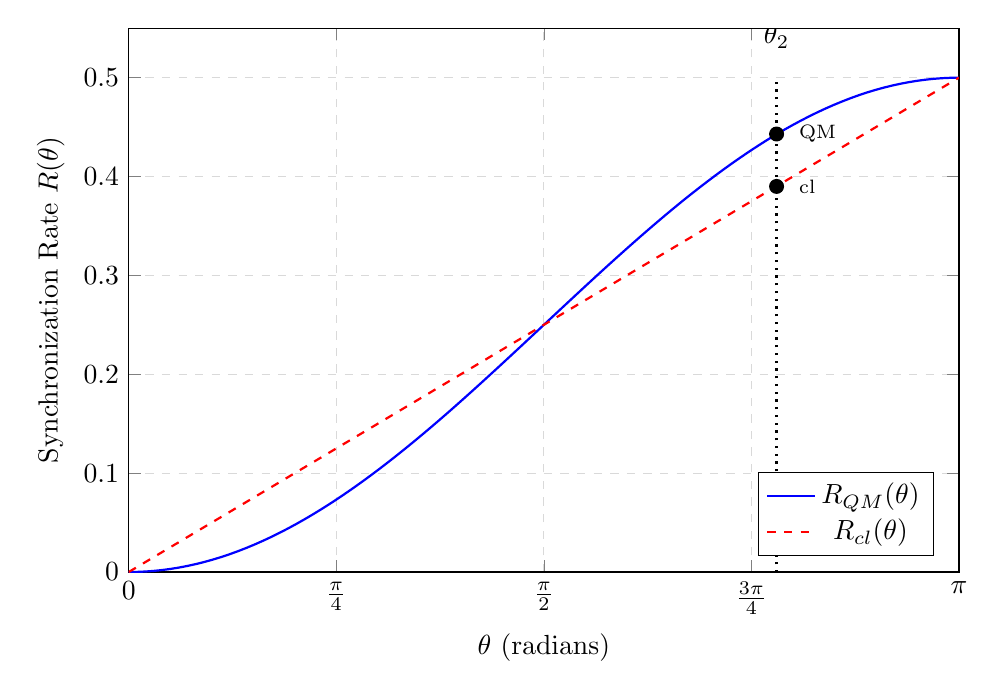
\begin{tikzpicture}
\begin{axis}[
    width=\columnwidth,
    height=0.7\columnwidth,
    xlabel={$\theta$ (radians)},
    ylabel={Synchronization Rate $R(\theta)$},
    xmin=0, xmax=3.14159,
    ymin=0, ymax=0.55,
    xtick={0, 0.785, 1.571, 2.356, 3.14159},
    xticklabels={$0$, $\frac{\pi}{4}$, $\frac{\pi}{2}$, $\frac{3\pi}{4}$, $\pi$},
    legend pos=south east,
    grid=major,
    grid style={dashed, gray!30},
]
% Quantum rate
\addplot[blue, thick, domain=0:pi, samples=100]
    {0.5*sin(deg(x/2))^2};
\addlegendentry{$R_{QM}(\theta)$}

% Classical rate
\addplot[red, thick, dashed, domain=0:pi]
    {x/(2*pi)};
\addlegendentry{$R_{cl}(\theta)$}

% Mark the critical points
\addplot[only marks, mark=*, mark size=2.5pt, black]
    coordinates {(2.4515, 0.443) (2.4515, 0.390)};

% Labels for markers
\node[anchor=west, font=\scriptsize] at (axis cs:2.5, 0.443) {QM};
\node[anchor=west, font=\scriptsize] at (axis cs:2.5, 0.390) {cl};

% Vertical line at theta_2
\draw[dotted, thick] (axis cs:2.4515,0) -- (axis cs:2.4515,0.5);
\node at (axis cs:2.4515,0.52) [anchor=south] {$\theta_2$};

\end{axis}
\end{tikzpicture}
\caption{Comparison of the quantum ($R_{QM}$, solid blue) and classical ($R_{cl}$, dashed red) synchronization rates as functions of the relative detector angle $\theta$. The curves coincide at $\theta = 0, \pi/2, \pi$ but diverge maximally at $\theta_2 \approx 140.5^\circ$, where the quantum clock ``ticks faster.''}
\label{fig:rates}
\end{figure}

The cosine modulation of the quantum correlation function, which is consistent with Zeilinger's information-invariance principle, permits a higher density of coincident events than the linear constraint imposed by the isotropic bomb-fragment model. In particular, at $\theta_2$ the quantum prediction exceeds the linear classical benchmark by about $13.6\%$.
Figure~\ref{fig:delta} explicitly shows this synchronization excess $\Delta(\theta)$. The positive lobe represents a regime where, if one demands a single local realistic model that applies to \emph{all} angles simultaneously, the quantum predictions force the clocks to agree more often than such a model can allow.

\begin{figure}[t]
\centering
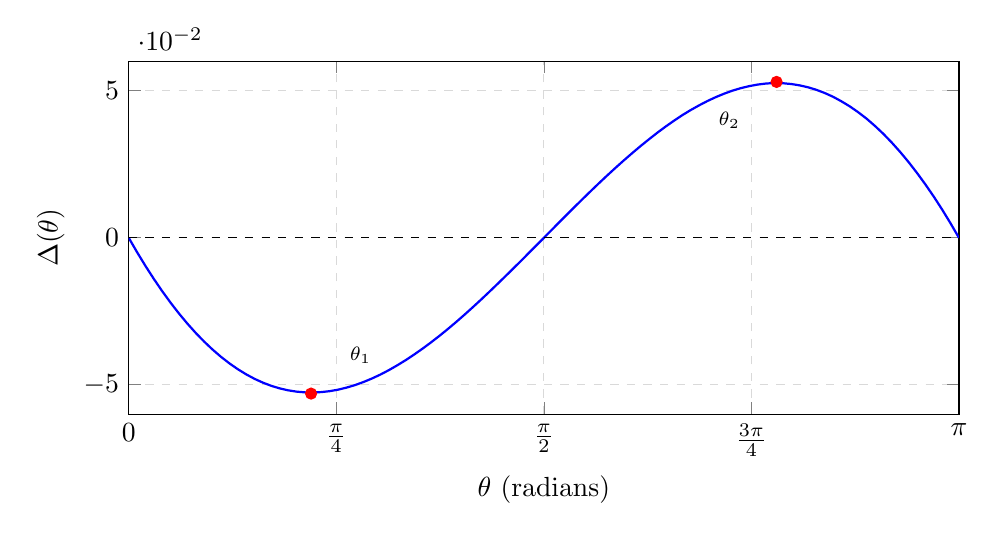
\begin{tikzpicture}
\begin{axis}[
    width=\columnwidth,
    height=0.5\columnwidth,
    xlabel={$\theta$ (radians)},
    ylabel={$\Delta(\theta)$},
    xmin=0, xmax=3.14159,
    ymin=-0.06, ymax=0.06,
    xtick={0, 0.785, 1.571, 2.356, 3.14159},
    xticklabels={$0$, $\frac{\pi}{4}$, $\frac{\pi}{2}$, $\frac{3\pi}{4}$, $\pi$},
    grid=major,
    grid style={dashed, gray!30},
]
\addplot[blue, thick, domain=0:pi, samples=100]
    {0.5*sin(deg(x/2))^2 - x/(2*pi)};
\draw[dashed, black] (axis cs:0,0) -- (axis cs:pi,0);
\addplot[only marks, mark=*, mark size=2pt, red]
    coordinates {(0.69, -0.053) (2.4515, 0.053)};
\node at (axis cs:0.8, -0.04) [anchor=west, font=\scriptsize] {$\theta_1$};
\node at (axis cs:2.35, 0.04) [anchor=east, font=\scriptsize] {$\theta_2$};
\end{axis}
\end{tikzpicture}
\caption{The synchronization excess $\Delta(\theta) = R_{QM} - R_{cl}$. The quantum clock lags at acute angles ($\theta_1 \approx 39.5^\circ$) but leads at obtuse angles ($\theta_2 \approx 140.5^\circ$).}
\label{fig:delta}
\end{figure}

\section{Contextuality and Unperformed Experiments}

Why does the quantum clock tick faster? The answer lies in the nature of the information carried by the system and the role of contextuality.

In Peres' model~\cite{peres222}, the angular momentum vector $\vec{J}$ exists independently of the measurement. Peres argues that Bell's inequality can be derived by constructing a table of outcomes for experiments actually performed (settings $\vec{a}, \vec{b}$) and hypothetical experiments \emph{not} performed (settings $\vec{a}', \vec{b}'$). For a classical system, this table must be internally consistent because the value $\vec{J}$ pre-exists and determines the outcome for any possible question. In the specific bomb-fragment model, the overlap of the corresponding hemispheres on the unit sphere yields a strictly linear correlation function, Eq.~\eqref{eq:peres_corr}, which in turn strictly limits the synchronized tick rate.

In the quantum case, following Zeilinger~\cite{zeil-99}, the bipartite system carries only 2 bits of information, which are already exhausted by the specific joint state. There is no ``spare'' information to encode definite answers to all possible, mutually incompatible measurement questions along directions $\vec{a}',\vec{b}'$. From this information-theoretic perspective, the system is not constrained to maintain consistency across a full table of actual and counterfactual outcomes, and thus is not subject to the Boole--Bell-type constraints~\cite{froissart-81,pitowsky-86} that enforce the existence of a single joint probability distribution for all settings and, in particular, lead to linear behavior in models like Peres' bomb. This ``freedom from counterfactual definiteness'' is one way to understand why the quantum correlation $E_{QM}(\theta)$ follows the cosine law and exceeds the linear bomb-model bound at $\theta \approx 140^\circ$.


\subsection{Certifying Quantumness}
While the rate $R_{QM} \approx 0.44$ is notably higher than the standard classical rate $R_{cl} \approx 0.39$, one must be cautious. A single measurement setting cannot distinguish quantum from classical clocks. As noted in recent work on contextuality~\cite{svozil-2022-epr}, for any \emph{single} fixed angle $\theta^*$, one can construct a local classical model (e.g., Aerts' ``broken elastic band'' model~\cite{aerts-69}) that reproduces the quantum probability $R_{QM}(\theta^*)$ exactly. In such models, the hidden variable space is deformed or the probability density is non-uniform to mimic the cosine statistics locally.

The signature of quantum synchronization is \emph{contextual}: the same underlying state produces the \emph{entire} cosine curve across all angles simultaneously. To certify quantumness, Alice and Bob must therefore vary their angles and compare several correlations at once. Any local realistic model must admit a single joint probability distribution that reproduces all these correlations and thus obeys Bell-type inequalities, whereas the quantum clock yields a family of cosine values that violates these bounds. The enhanced synchronized tick rate in the obtuse regime is then seen not as an isolated anomaly, but as one facet of a globally nonclassical correlation structure.

The excess synchronization rate $\Delta(\theta) > 0$ in the obtuse regime is directly related to violations of Bell-type inequalities such as the Clauser--Horne--Shimony--Holt (CHSH) inequality~\cite{chsh}.
The CHSH parameter $S$ is composed of four correlation terms:
\begin{equation}
S = |E(\vec{a},\vec{b}) - E(\vec{a},\vec{b}') + E(\vec{a}',\vec{b}) + E(\vec{a}',\vec{b}')|.
\end{equation}
The classical bound $S \le 2$, obtained from the convex hull computation of the corresponding correlation polytope~\cite{froissart-81,pitowsky-86}, arises from the requirement that all four correlations be marginals of a single joint probability distribution, that is, from the assumption that the table of actual and counterfactual outcomes is internally consistent.
The linear correlation function~\eqref{eq:peres_corr} is one explicit realization of such a local realistic model.
The quantum violation (approaching the Tsirelson bound $2\sqrt{2}$) and the enhanced synchronization rate in the obtuse regime are two manifestations of the same underlying phenomenon.

\section{Experimental Considerations}

Implementing this protocol requires addressing practical constraints. In an ideal scenario, every particle pair results in a potential tick. In reality, photon detectors have finite efficiency $\eta < 1$.

If $\eta < 1$, the clocks will frequently ``miss'' ticks even when the quantum outcome would have been $+1$. However, the synchronization rate $R(\theta)$ is typically measured as a coincidence rate normalized by the total number of emitted pairs (or inferred from singles counts). If we define the measured rate $R_{exp}(\theta)$, we have:
\begin{equation}
R_{exp}(\theta) \approx \eta_A \eta_B R_{QM}(\theta).
\end{equation}
This reduced efficiency lowers the absolute rate of ticking for both classical and quantum models. The crucial comparison is the \emph{relative} rate or the visibility of the interference fringe. A high-visibility experiment (using, for example, spontaneous parametric down-conversion and superconducting nanowire single-photon detectors with $\eta > 0.9$) would clearly resolve the difference between the linear classical prediction and the sinusoidal quantum prediction.

Furthermore, the definition of ``simultaneity'' requires a coincidence window $\tau_c$. If the path lengths to Alice and Bob differ, or if there is electronic jitter, ticks might not register as simultaneous. Standard quantum optical techniques allow $\tau_c$ to be on the order of nanoseconds. The ``Entangled Clock'' is thus a statistical construct: it does not provide a continuous readout for a single run but establishes a time scale over an ensemble of events, where the density of synchronized events serves as the metrological standard.

\section{Conclusion}

We have proposed an operational protocol in which spatially separated quantum clocks, synchronized via singlet-state correlations, exhibit a measurable enhancement in their coincidence rate compared to Peres-type classical mechanisms based on conserved angular momentum and, more generally, to any local realistic model once correlations at several measurement angles are taken into account. By unifying the ``single-unit universe'' concept with an information-theoretic view of quantum randomness, we showed that the ``bona fide clock'' fixing the metric scale is locally random but relationally structured.

At a relative measurement angle of $\theta \approx 140^\circ$, this ``temporal speedup'' in the synchronized tick rate reaches ${\sim}13\%$ relative to the linear bomb-model benchmark. The effect traces to contextuality: quantum systems need not maintain consistency with unperformed measurements, freeing the correlation function from the linear constraints of specific hidden-variable models. Certification of this quantum advantage requires Bell-type inequality tests across multiple measurement contexts---similar to private randomness~\cite{Acin2016CertifiedRandomness}---confirming that the cosine modulation cannot be replicated by any local realistic mechanism. In this sense, the entangled clock embodies the informational character of quantum time: random in isolation, relational in synchrony, and---when judged against the full set of classical constraints---faster than classical physics permits.


\begin{acknowledgments}
The entangled clock metaphor was suggested by Adrienne Toman during a hike to the Michelberg.

This research was funded in whole or in part by the Austrian Science Fund (FWF) Grant DOI: 10.55776/PIN5424624. The author acknowledges TU Wien Bibliothek for financial support through its Open Access Funding Programme.
\end{acknowledgments}

\bibliography{svozil}

\end{document}


expose

tentativer title: quantum clocks tick faster

* intro section on recent developments (input manuscript I)

* prime section: compare two readings of an ``entangled clock'' on different spatial locations.  Singlet state of two photos or electrons.

Whenever the outcome records an ``up'' click, the clock adds ``1'' to the time counter.

** readdoff: number of ``up'' readings determines time on each side. ``synchronicity'' is depending on the relative

** consider perfect opposite direction reading observables (detectors \pi apart): clocks will be in perfect synchrony.
** consider perfect same direction reading observables (detectors 0 apart): clocks will be in perfect anti-synchrony.
** consider perfect unbiuased direction reading observables (detectors \pi/2 apart): clocks will be in perfect non-correllation.
** in all those cases single events and outcomes on either one side will occur totally random, as entanglement is defined vie relational encoding (cf. Zeilinger's foundational principle, paper enclosed)

in the there ``special'' cases this is also possible classically; cf. Peres' bomb explosion example.

*** now consider relative measurement angles not equal to the ``special cases'' 0, Pi/2 and \pi, but, say, somewhere in-between \pi/2 and \pi; ideally at an angle that maximises  the absolute difference between quantum and classical (linear) correllation) for a Bell basis singlet state---please compute.

** in such a case the clocks on both sides will record ``more'' clicks than ``usual classical clocks clocks'', because of the difference between classical and quantum correllations.
Same could be done with a reagin between relative angle 0 and \pi/2, only the time measures is less that the classical time recorden.

New section: not so fast! However for SINGLE unique relative measurement angle measurement the cosine correlation function can be reproduced classically---cf Aerts' rubber band model. But not for 4 direwctions and 4 measurement contexts, as is the case for the CHSH ineaquality.

So only if more contexts are taken into account, Bell-type inequalities could assure ``quantumness'' of  the clock readings.

